\documentclass{article}
\usepackage{graphicx}
\usepackage{polski}
\usepackage{enumerate}

\title{Lista 1}
\author{Maciej Kmieciak, 277516}
\date{11.2024}

\begin{document}

\maketitle

\section{Wstęp}

Do zaimplementowania były trzy algorytmy sortujące: Insertion Sort, Merge Sort oraz Heap Sort. Następnie należało każdy z nich zmodyfikować. Insertion Sort w nowej odsłonie miał wstawiać "na raz" dwa kolejne elementy tablicy. Modyfikacja Merge Sort polegała na dzieleniu na trzy części zamiast dwóch. Z kolei Heap Sort miał tworzyć kopce ternarne zamiast binarnych.

W każdym z algorytmów trzeba było dodać zmienne liczące porównania i przypisania. Dzięki uzyskanym w ten sposób danym można porównać zaimplementowane algorytmy.

Program wypełnia coraz większe tablice (do wielkości 10000) losowymi liczbami, a następnie sortuje je każdym z algorytmów. Wyniki, czyli liczby porównań i przypisań, wypisywane są w konsoli oraz zapisywane w pliku z rozszerzeniem \texttt{.csv}, który służy jako źródło danych dla wykresu. Dla poprawy czytelności, wykres został wykonany w skali logarytmicznej.

\section{Najciekawsze fragmenty kodu}

Poniżej znajdują się kluczowe fragmenty zmodyfikowanych wersji algorytmów. Tutaj usunięto z nich liczniki porównań i przypisań.

\subsection{Modyfikacja Insertion Sort}

\begin{verbatim}
for (int i = 1; i + 1 < n; i += 2) {
    if (A[i] > A[i + 1]) {
        swap(A[i], A[i + 1]);
    }

    int x = A[i], y = A[i + 1];

    int j = i - 1;
    int k = i;
    while (j >= 0 && k >= 0 && A[j] > x) {

        A[j + 1] = A[j];
        --j;

        if (A[k] > y) {
            A[k + 1] = A[k];
            --k;
        }
    }

    A[j + 1] = x;
    A[k + 1] = y;
}
\end{verbatim}

W pętli \texttt{for} przesuwamy się co dwa indeksy, ponieważ wstawiamy dwa elementy na raz. Musimy sprawdzić, czy one same są posortowane, a jeśli nie, zamienić je miejscami. Tworzymy dwie zmienne: \texttt{j} i \texttt{k}, przechowujące odpowiednio indeks do wstawienia pierwszej i drugiej liczby z pary. Następnie postępujemy, jak w zwykłym Insertion Sort, z tą różnicą, że po porównaniu z pierwszą liczbą z pary i dostosowaniu indeksu \texttt{j}, porównujemy jeszcze z drugą liczbą z pary i przesuwamy dalej "w prawo", jeśli trzeba, zmniejszając indeks \texttt{k}.

\subsection{Modyfikacja Merge Sort}

\begin{verbatim}
int n1 = part1 - p + 1;
int n2 = part2 - part1;
int n3 = k - part2;

int* L = new int[n1 + 1];
int* M = new int[n2 + 1];
int* R = new int[n3 + 1];

L[n1] = high + 1;
M[n2] = high + 1;
R[n3] = high + 1;

for (int i = 0; i < n1; ++i) L[i] = A[p + i];

for (int j = 0; j < n2; ++j) M[j] = A[part1 + 1 + j];

for (int l = 0; l < n3; ++l) R[l] = A[part2 + 1 + l];

int i = 0, j = 0, l = 0;

for (int m = p; m <= k; ++m) {
    if (L[i] <= M[j] && L[i] <= R[l]) {
        A[m] = L[i];
        i++;
    }
    else if (M[j] <= L[i] && M[j] <= R[l]) {
        A[m] = M[j];
        j++;
    }
    else {
        A[m] = R[l];
        l++;
    }
}
\end{verbatim}

To fragment, w którym łączymy trzy posortowane części w jedną, która również będzie posortowana. W ostatniej pętli \texttt{for} szukamy najmniejszej liczby z porównywanej trójki i wstawiamy ją do wynikowej tablicy, jednocześnie inkrementując indeks odpowiadający fragmentowi, w którym ją znaleziono (tzn. mniejszej tablicy, jednej z trzech), tak aby w kolejnej iteracji porównywać z kolejną w nim liczbą.

\subsection{Modyfikacja Heap Sort}

\begin{verbatim}
void heapify_mod(int A[], int i, int size) {
    int largest = i;
    int left = 3 * i + 1;
    int middle = 3 * i + 2;
    int right = 3 * i + 3;
    
    if (left < size && A[left] > A[largest]) largest = left;

    if (middle < size && A[middle] > A[largest]) largest = middle;

    if (right < size && A[right] > A[largest]) largest = right;

    if (largest != i) {
        swap(A[i], A[largest]);
        heapify_mod(A, largest, size);
    }
}
\end{verbatim}

W Heap Sort po modyfikacji musimy uwzględnić fakt, że każdy rodzic ma trójkę, a nie dwójkę dzieci. Obliczając miejsce (indeks) dziecka w tablicy, dzielimy przez 3, a szukając największego dziecka (aby potem porównać je z rodzicem i zamienić miejscami, jeśli trzeba), musimy porównać ze sobą wszystkie trzy wartości.

\section{Porównanie działania algorytmów}

\subsection{Liczba przypisań}

Liczba przypisań dla różnych rozmiarów tablicy:

\begin{center}
\begin{tabular}{|c|c|c|c|c|}
 \hline
 n & Ins. Sort & Ins. Sort Mod. & Merge Sort & Merge Sort Mod. \\ 
 \hline
 10 & 73 & 76 & 165 & 121 \\
 100 & 4877 & 4902 & 2709 & 1963 \\
 1000 & 491575 & 491819 & 36921 & 26611 \\
 10000 & 49919281 & 49921780 & 470841 & 334543 \\
 \hline
\end{tabular}

\vspace{0.5cm}

\begin{tabular}{|c|c|c|c|}
 \hline
 n & Heap Sort & Heap Sort Mod. \\ 
 \hline
 10 & 198 & 182 \\
 100 & 4331 & 3593 \\
 1000 & 67953 & 54341 \\
 10000 & 927354 & 725681 \\
 \hline
\end{tabular}
\end{center}

\begin{center}
    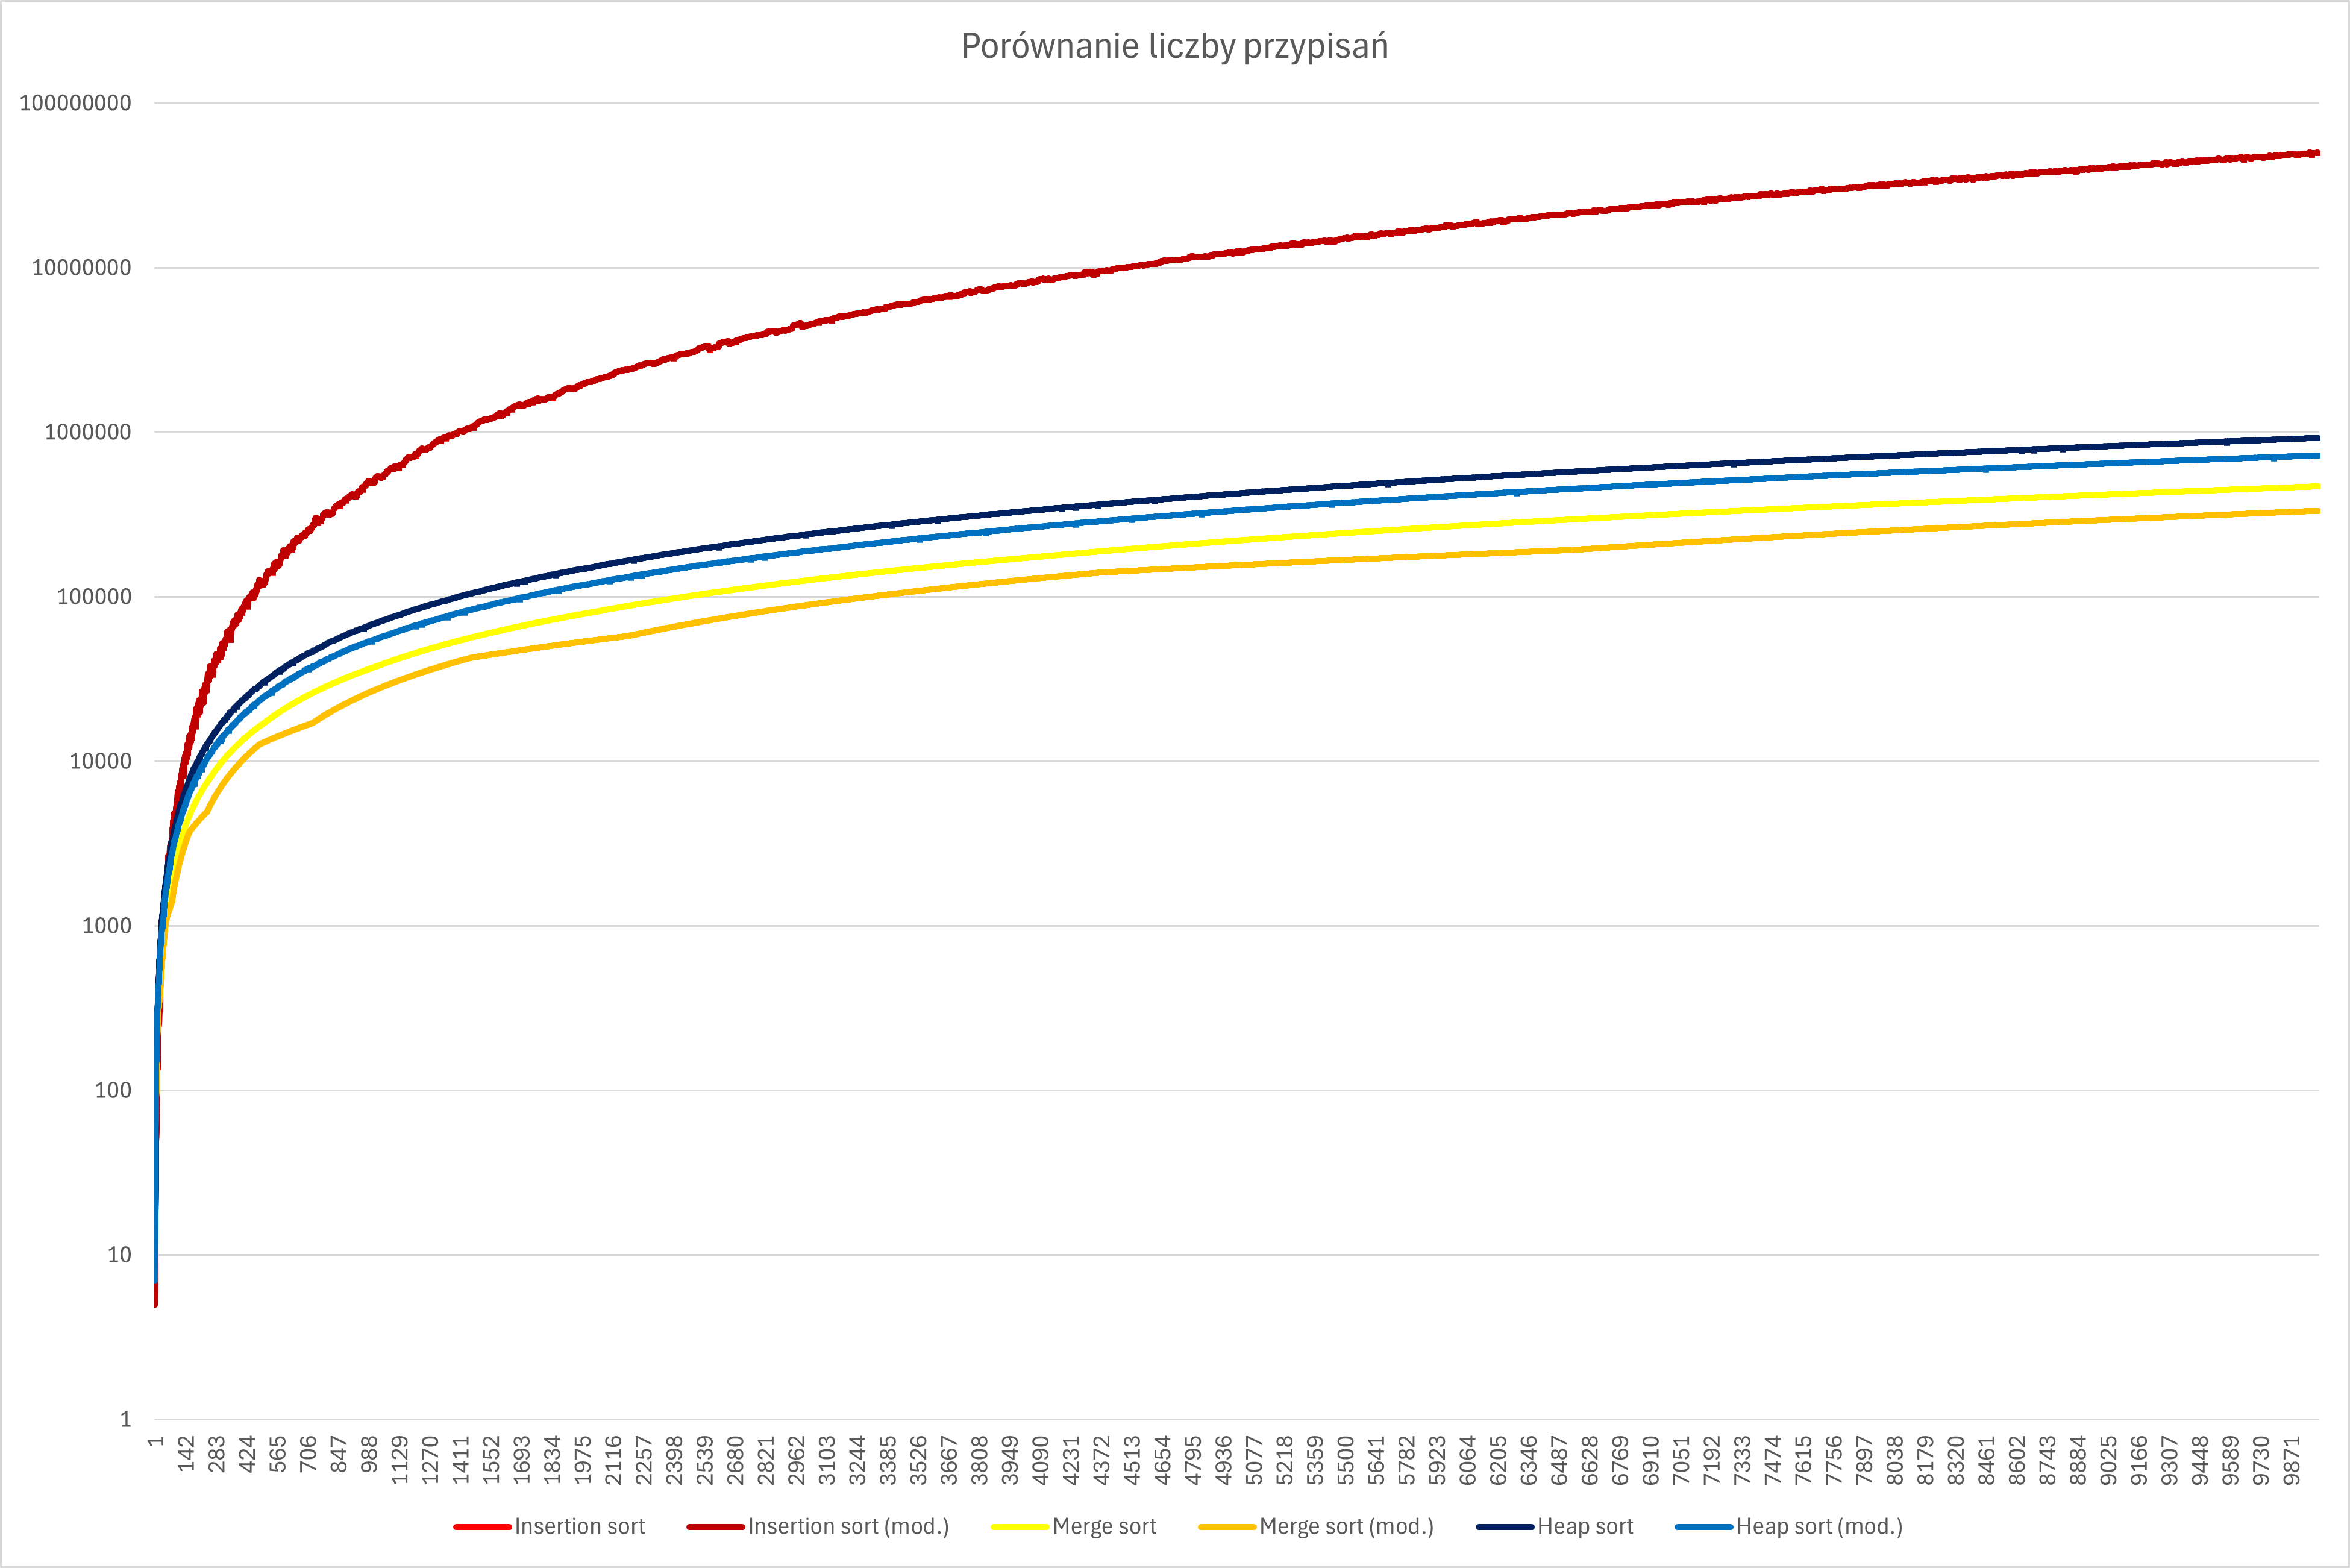
\includegraphics[width=1\textwidth]{Wykres1.png}
\end{center}

\subsection{Liczba porównań}

Liczba porównań dla różnych rozmiarów tablicy:

\begin{center}
\begin{tabular}{|c|c|c|c|c|}
 \hline
 n & Ins. Sort & Ins. Sort Mod. & Merge Sort & Merge Sort Mod. \\ 
 \hline
 10 & 32 & 31 & 53 & 75 \\
 100 & 2389 & 3102 & 871 & 1356 \\
 1000 & 245288 & 326808 & 11975 & 19356 \\
 10000 & 24954641 & 33379757 & 153615 & 252710 \\
 \hline
\end{tabular}

\vspace{0.5cm}

\begin{tabular}{|c|c|c|c|}
 \hline
 n & Heap Sort & Heap Sort Mod. \\ 
 \hline
 10 & 117 & 116 \\
 100 & 2576 & 2333 \\
 1000 & 40614 & 35477 \\
 10000 & 554472 & 475187 \\
 \hline
\end{tabular}
\end{center}

\begin{center}
    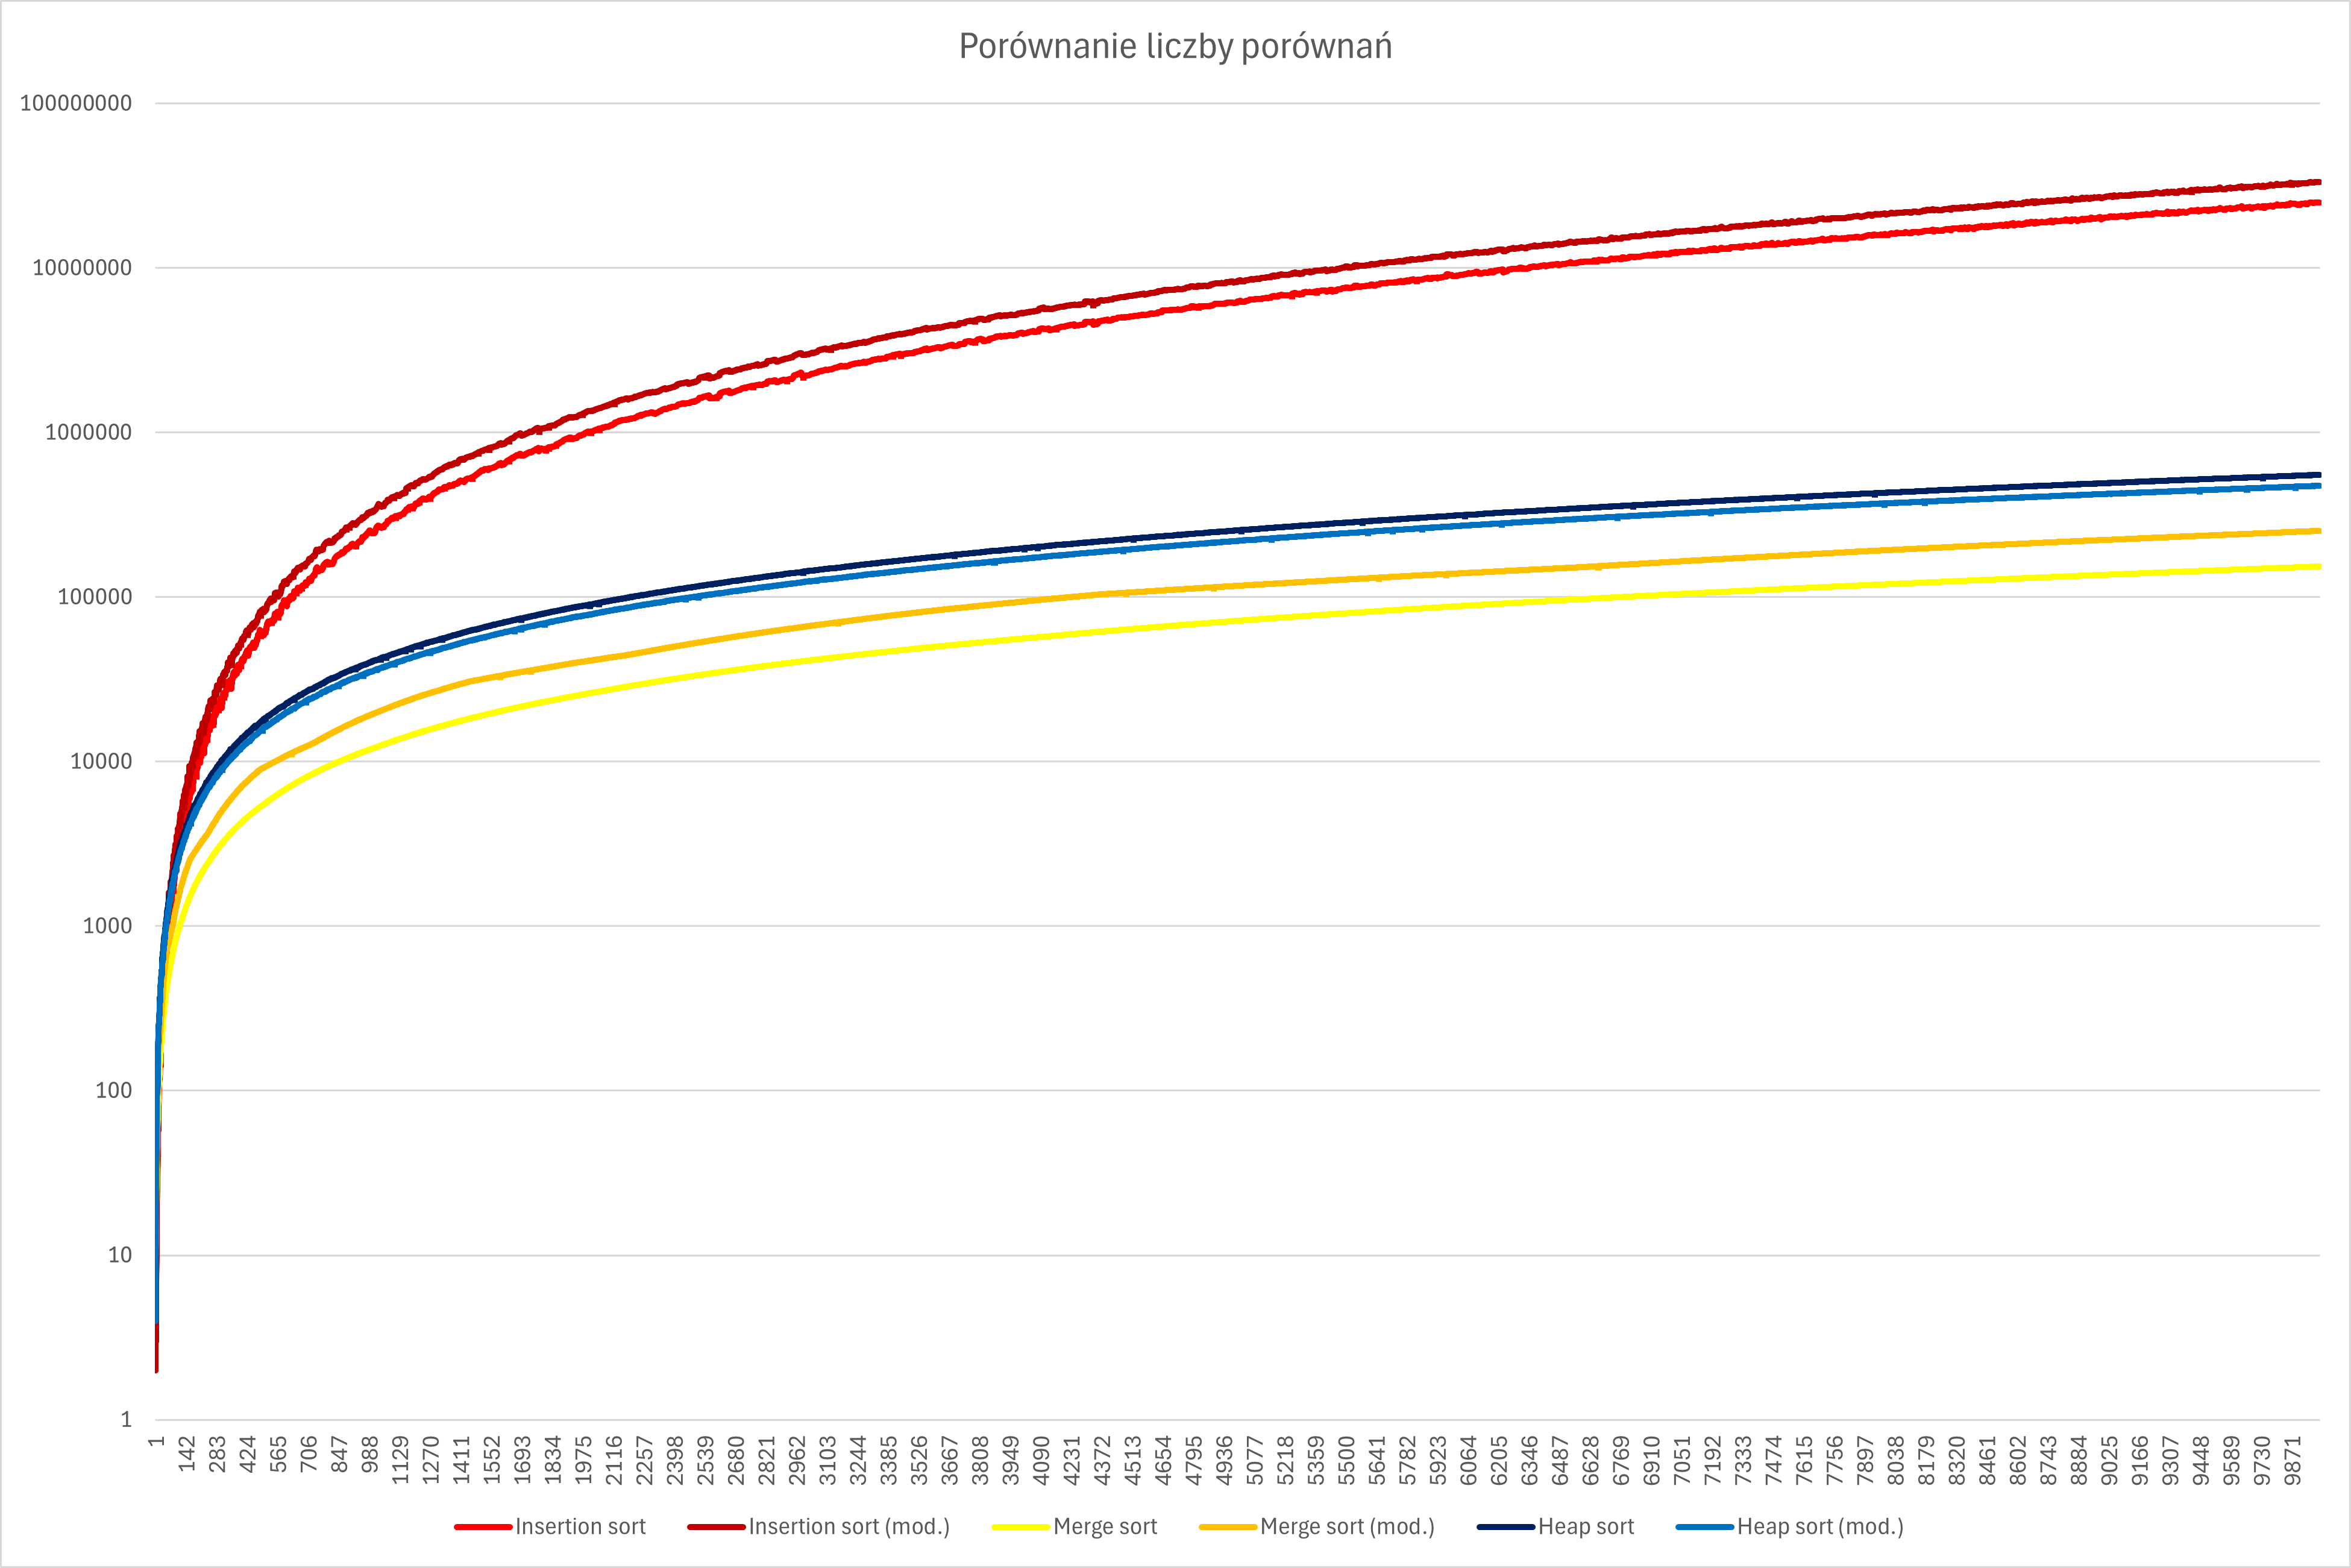
\includegraphics[width=1\textwidth]{Wykres2.png}
\end{center}

\section{Wnioski}

\subsection{Który algorytm jest najszybszy?}

Na podstawie danych można stwierdzić, że zdecydowanie najwolnieszym algorytmem, zarówno pod względem liczby porównań, jak i przypisań, jest Insertion Sort (kolor czerwony na wykresie). Drugim z kolei jest Heap Sort (kolor niebieski), a trzecim - najszybszym - Merge Sort (kolor żółty). Na przykład, dla tablicy o rozmiarze 10000, Heap Sort wykonał w przybliżeniu 3,61 raza więcej porównań niż Merge Sort, a Insertion Sort aż 162 razy więcej. 

\subsection{Jak modyfikacja wpłynęła na wydajność algorytmów?}

Dla Insertion Sort nie wydać istotnej różnicy w liczbie przypisań, a liczbę porównań jest większa dla zmodyfikowanej wersji. Dla Heap Sort, modyfikacja zmniejszyła zarówno liczbę porównań, jak i przypisań, mamy więc poprawę wydajności. Z kolei dla Merge Sort, wersja dzieląca na trzy części, zamiast dwóch, wykonuje mniej przypisań, lecz więcej porównań - nie jest zatem jasne, który wariant jest lepszy.

\subsection{Dodatkowa obserwacja}

Przyglądając się wykresom można też zauważyć większe wahania liczby przypisań i porównań w przypadku zmodyfikowanej wersji Merge Sort. Pomarańczowa linia jest bardziej "pofalowana" niż pozostałe, szczególnie dla \(n \in [500, 3000]\), co może oznaczać większy wpływ danych w tablicy na czas działania algorytmu.

\end{document}
